% Metódy inžinierskej práce

\documentclass[10pt,oneside,slovak,a4paper]{article}

\usepackage[slovak]{babel}
\usepackage[T1]{fontenc}
\usepackage[IL2]{fontenc} % lepšia sadzba písmena Ľ než v T1
\usepackage[utf8]{inputenc}
\usepackage{graphicx}
\usepackage{url} % príkaz \url na formátovanie URL
\usepackage{hyperref} % odkazy v texte budú aktívne (pri niektorých triedach dokumentov spôsobuje posun textu)

\usepackage{cite}
%\usepackage{times}

\pagestyle{headings}

\title{Evolúcia počítačových hier, videohier a ich rozdelenie podľa žánrov\thanks{Semestrálny projekt v predmete Metódy inžinierskej práce, ak. rok 2022/23, vedenie: Ing. Ivan Kapustík}} % meno a priezvisko vyučujúceho na cvičeniach

\author{Dávid Babiš\\[2pt]
	{\small Slovenská technická univerzita v Bratislave}\\
	{\small Fakulta informatiky a informačných technológií}\\
	{\small \texttt{xbabis@stuba.sk}}
	}
	

\date{\small 17.10.2022}



\begin{document}

\maketitle

\begin{abstract}
 V tomto článku sa dozviete niečo o histórii videohier a počítačových hier od roku 1947. Rozdiel je naozaj obrovský. Pozrieme sa aj na ich rozdelenie, a rozdelíme si ich do základných žánrov. Porovnáme si aj dve známe strielačky Counter-Strike 1.6 a Counter-Strike: Global Offensive. Pamätáte si ešte niektoré staré klasiky?
\end{abstract}



\section{Úvod}
Ak sa chcete dozvedieť viac o vývine hier, a ich rozdelení, ste tu na správnom mieste. V tomto článku sa spoločne pozrieme na videohry, počítačové hry, ich históriu a rozdelenie podľa žánrov. Tiež si porovnáme starú a novú verziu jednej kultovej hry, a ukážeme si ako sa časom z hľadiska mechaniky a grafiky zmenila. V závere si tento pokrok ešte zhrnieme. História pc hier naznačená v úvode, je podrobnejšie vysvetlená v časti~\ref{historia}. Porovnanie zmien v konkrétnej videohre nájdete v časti~\ref{porovnanie}. 
Dôležité súvislosti s rozdelením videohier podľa žánrov sú uvedené v časti~\ref{zanre}. Reakcia na témy z prednášok sa nachádza v časti~\ref{reakcia}. 
Záverečné poznámky prináša časť~\ref{zaver}.

\pagebreak

\section{História počítačových hier a videohier} \label{historia}
Vedeli ste že rok 1947 je považovaný za rok zvniku prvej videohry?. V tejto časti si ukážeme tie najdôležitejšie a najrevolučnejšie videohry, ale aj prvé herné konzoly. Článok, ktorý bližšie vysvetluje túto tému\cite{Lowood}. Evolúcia digitálnych hier je podrobnejšie vysvetlená v štúdii\cite{sahay}.

\subsection{Prvé videohry}

V roku 1952 vyvinul Alexander Shafto "Sandy" Douglas videohru OXO(obrázok~\ref{oxo}, zdroj\footnote{http://www.warpedfactor.com/2015/09/video-game-firsts-oxo.html}). Bola to grafická verzia známej hry piškvorky. Hra bola nainštalovaná na elektrónkovom počítači EDSAC, ktorý bežne používal dierne pásky. Zobrazenie bitmapy bolo 35×16 pixelov. Hralo sa len proti umelej inteligencii. Hra sa ovládala pomocou vytáčacieho telefónu.

\begin{figure*}[tbh]
\centering
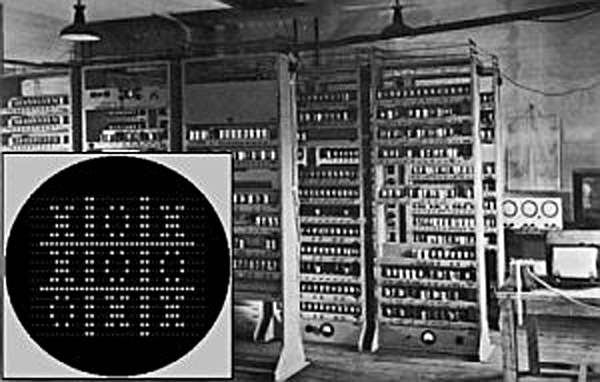
\includegraphics[scale=0.3]{oxo.jpg}
\caption{V pozadí EDSAC, v ľavom dolnom rohu obrazovka s výstupom hry.}
\label{oxo}
\end{figure*}

Ďalšia videohra sa nazýva Tennis For Two. Vynašiel ju William Higinbotham v roku 1958. Hra spočívala v tom, že na obrazovke bol zobrazený zboku tenisový kurt(obrázok~\ref{tenis}, zdroj\footnote{https://www.geekzone.fr/2017/01/26/tennis-for-two-higinbotham-inventa-jeu-video/}), a dvaja hráči pomocou dvoch veľkých ovládačov(obrázok~\ref{tenis2}, zdroj\footnote{https://www.evilmadscientist.com/2008/resurrecting-tennis-for-two-a-video-game-from-1958/}) si medzi sebou odrážali lotpu. Na ovládačoch boli dve tlačidlá. Jeden pre ovládanie trajektórie a druhý pre odpálenie lopty.

\begin{figure*}[tbh]
\centering
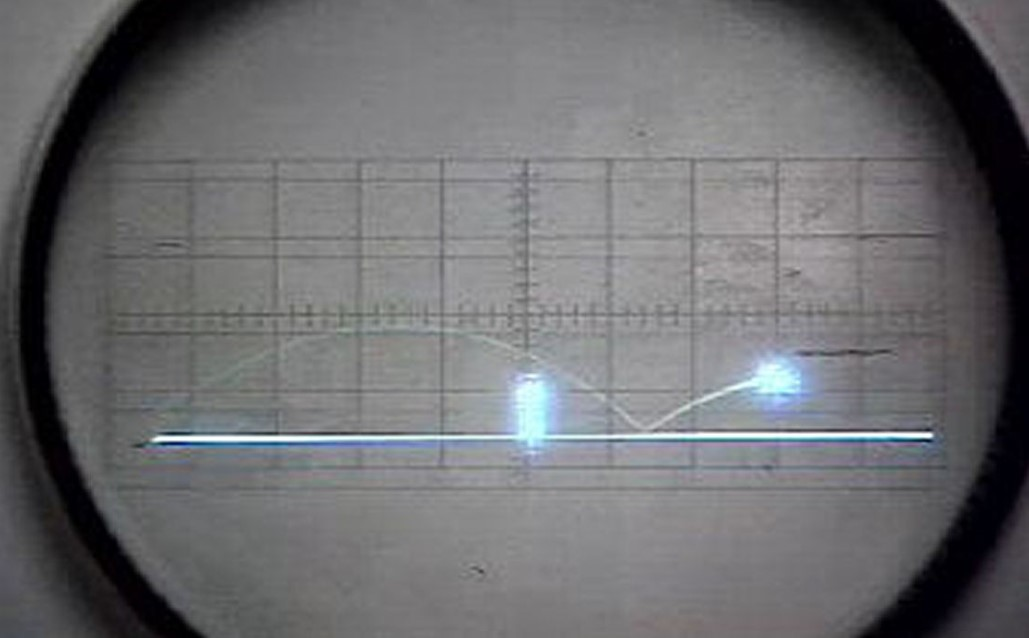
\includegraphics[scale=0.25]{tenis.jpg}
\caption{Obrazovka na ktorej je vidno tenisový kurt zboku a loptu.}
\label{tenis}
\end{figure*}

\begin{figure*}[tbh]
\centering
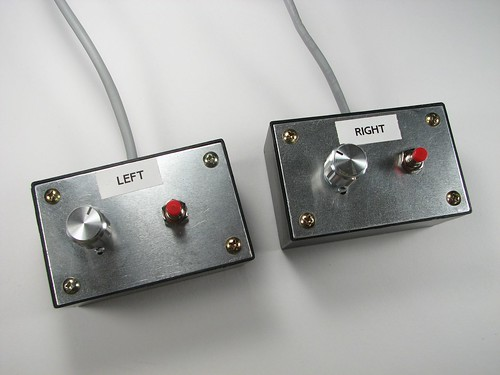
\includegraphics[scale=0.35]{tenis2.jpg}
\caption{Ovládače na ovládanie hry.}
\label{tenis2}
\end{figure*}

\subsection{Šesťdesiate a sedemdesiate roky} \label{sedemdesiate}

Veľa hier zo šesťdesiatych rokov bolo vytvorených študentmi na univerzitách v Amerike. 

V roku 1961 vznikla hra Spacewar. Hra bola pre dvoch hráčov a každý z nich ovládal vlastnú vesmírnu loď, ktorá dokázala strieľať rakety. Cieľom bolo zničiť druhého hráča.

V roku 1969 vytvoril Ralph Baer prototyp hernej konzoly. Dala sa pripojiť k televízii a bolo v nej pár hier. Spoločnosť Magnavox túto konzolu odkúpila a v roku 1972 ju vydala. Volala sa Odyssey.

Nolan Bushnell a Ted Dabney vytvorili v roku 1971 verziu hry Spacewar na hracom automate. Volala sa Computer Space. Odkúpila ju spoločnosť Nutting Associates a začala vyrábať automaty. Hra bola veľmi obtiažna a preto nemala až tak veľký úspech.

V roku 1972 založil Nolan Bushnell spoločnosť Atari a vytvoril hru Pong. Hra bola pre dvoch hráčov, každý ovládal jednu plošinu, ktoré ležali oproti sebe. Pomocou plošín odrážali loptičku. Cieľom hry bolo odraziť loptičku tak, aby ju druhý hráč nechytil. "Pong bola jednoduchá hra, čo bola jednoznačná konkurenčná výhoda pre arkádové hry, ktoré sa často umiestňovali v baroch a reštauráciách, kde mohol patrón hrať s drinkom v jednej ruke."\cite{Lowood}

V roku 1976 vyšla hra Death Race. Cieľom bolo autom zrážať goblinov. Death Race vyvolala rozruch v spoločnosti kvôli násiliu.

Spoločnosť Taito Vydala v roku 1978 arkádu Space Invaders. Bola to pevná strieľačka. Cieľom hry bolo zastreliť všetkých mimozenšťanov. Hráč strieľal z dela, ktoré sa pohybovalo v spodnej časti obrazovky. Touto hrou začína v USA zlatý vek herných automatov.

V roku 1979 vydala spoločnosť Atari populárnu hru Asteroids. Hráč ovládal vesmírnu loď a jeho cieľom bolo prežiť čo najdlhšie, a to pomocou strieľania asteroidov.

\pagebreak

\subsection{Osemdesiate roky} \label{osemdesiate}
V roku 1980 prišla na svet hra Battlezone, využívajúca vektorovú grafiku k skutočnému 3D zobrazeniu. Hráč riadil tank pomocou joystickov. Cieľom hry bolo zničiť ostatné tanky.

Japonský vydavaťeľ Namco vydal v roku 1980 hru Pac-Man. Išlo o veľmi obľúbenú arkádu, a stala sa jednou z najdlhšie fungujúcich a najpredávanejších videohier na svete. Hráč ovládal žltú guličku, pohyboval sa v bludisku a jeho cieľom bolo zjesť všetky bodky rozmiestnené po bludisku. Nepriateľom boli štyria duchovia, ktorí keď sa dotkli hráča tak hra skončila. V tejto štúdii sa písalo viac o fungovaní videohry Pac-Man\cite{SRVSS20}.

3D Monster Maze je hororová počítačová hra o prežitie vydaná vydavateľom JK Greye v roku 1981. Hráč mal za úlohu utekať pred dinosaurom po bludisku, za čo získaval body. Obtiažnosť sa postupne zvyšovala a keď dinosaurus chytil hráča, hra sa skončila.

V roku 1983 vydala spoločnosť Advanced Microcomputer Systems hru Dragon's Lair. Hráč hral za hrdinskú postavu Dirk the Daring. Cieľom hry bolo zachrániť princeznú Daphne pred zlým drakom Singe. Príbeh bol dopredu daný a hráč mal obmedzený vplyv na príbeh. Hra pozostávala z animovaných scén, kde mal hráč v správnom čase vykonať nejakú akciu stlačením tlačidla.

\subsection{Deväťdesiate roky až súčasnosť} \label{devatdesiate}
V roku 1992 vyšla Dune 2, hra, ktorá otvorila cestu pre ďalšie neskôr veľmi známe hry ako Command and Conquer či Warcraft. Dune 2 vydala spoločnosť Virgin Interactive. Hráč prevezme úlohu veliteľa jedného z troch medziplanetárnych domov, Atreidov, Harkonnenov alebo Ordovcov, s cieľom získať kontrolu nad planétou Arrakis.

Ďalej sa už akoby roztrhlo vrece s počítačovými hrami, a pribúda ich neskutočné množstvo.

\section{Porovnanie CS 1.6 a CS:GO} \label{porovnanie}

Akčnú FPS hru Counter-Strike asi netreba nikomu predstavovať. Legendárna hra ktorú si obľúbili milióny hráčov vznikla ako modifikácia hry Half-Life ešte v roku 1999. Od tej doby hra prešla mnohými úpravami. Ako samostatná hra vyšla v roku 2003 s názvom Counter-Strike 1.6 . Poďme sa teda spoločne pozrieť ako sa zmenila nielen po grafickej stránke v priebehu rokov. Budeme porovnávať jej úplne prvú verziu CS 1.6, s tou najnovšou, a to je Counter-Strike: Global Offensive (2012). Tak poďme sa nato pozrieť.


\subsection{Engine} \label{porovnanie:engine}
Zatiaľ čo 1.6 bežala na engine GoldSrc, CS:GO beží na engine Source od Valve Coproration. Source 3D engine bol vytvorený spoločnosťou Valve Software v roku 2004. Primárne bol určený pre hru Half-Life 2. Jeho základom bol predchádzajúci engine GoldSrc, čo bola silne upravená verzia Quake engine.

\pagebreak

Engine a jeho verzie Counter-Strikeu:
\begin{enumerate}
\item Engine GoldSrc
	\begin{enumerate}
	\item Couter-Strike Beta 1 - 7
	\item Couter-Strike 1.0 - 1.6
	\item Couter-Strike: Condition Zero (CS:CZ)
	\end{enumerate}
\item Engine Source
	\begin{enumerate}
	\item Couter-Strike: Source (CS:S)
	\item Couter-Strike: Global Offensive (CS:GO)
	\end{enumerate}
\end{enumerate}



\subsection{Grafika} \label{porovnanie:grafika}

Už na prvý pohľad vieme rozlíšiť CS 1.6 a CS:GO. Grafika 1.6 bola na svoju dobu veľmi pokroková. V denšnej dobe je grafika  CS:GO na vysokej úrovni a dokáže konkurovať aj ostatným kvalitným videohrám. Dnešná grafika je už skoro na nerozoznanie od reality, ale je to skutočne pravda? Toto isté si hovorili aj hráči na konci deväťdesiatych rokov keď zbadali CS 1.6 . Uvidíme ako to bude s hernou grafikou v budúcnosti. Pri súčašných technológiách ako je napríklad virtuálna realita je len otázkou času, kedy naozaj nerozoznáme hru od reality. Určite sa máme na čo tešiť. Obrázok s porovnaním grafiky CS 1.6 a CS:GO (obrázok~\ref{f:grafika}, zdroj\footnote{https://sazkaeleague.cz/article/video-herni-predmet-nebo-deset-fabii-cinsky-sberatel-skinu-ma-jasno}).

\begin{figure*}[tbh]
\centering
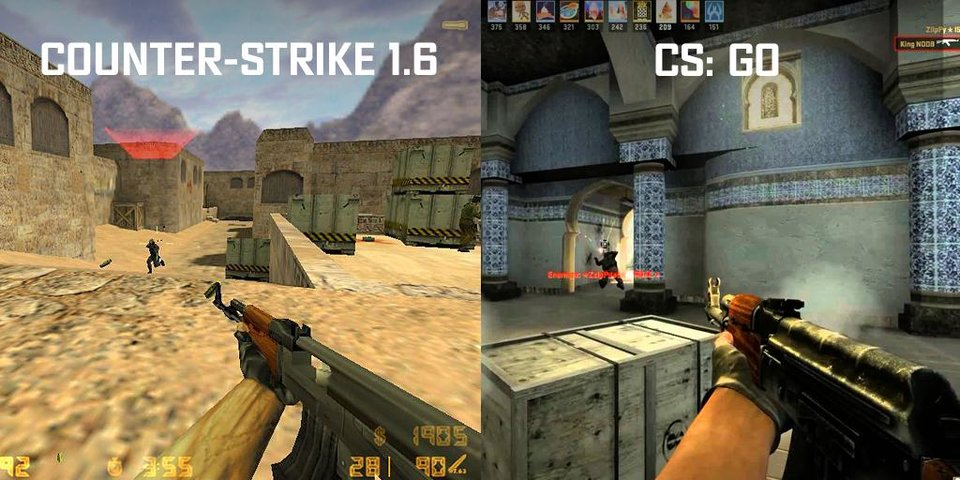
\includegraphics[scale=0.4]{1.6vsgo.jpg}
\caption{Porovnanie grafiky}
\label{f:grafika}
\end{figure*}

\subsection{Skiny} \label{porovnanie:skiny}

Zatiaľ čo CS 1.6 nemala mnoho skinov\footnote{vzhľadov na zbrane} na zbrane a boli väčšinou iba výsadov niektorých serverov, CS:GO ich má tisíce a stále pribúdajú. Ich hodnota sa vyjadruje v reálnych peniazoch, ale pritom ide o virtuálnu položku v počítači. Ich cena závisí od množstva existijúcich skinov alebo od krásy jednotlivého skinu. Vzácnych skinov je málo a preto sú aj oveľa drahšie. Skiny sa dajú kupvať a predávať anonymne cez virtuálny obchod Steamu, alebo aj vymieňať s ostatnými hráčmi.
Skiny sa dajú zadarmo získať  po každej hre, alebo si ich musí hráč kúpiť cez Steam market alebo od iného hráča. Skiny môže hráč ešte získať z debien, na ktorých odomknutie je treba virtuílny kľúč, ktorý ale nie je zadarmo. Hráč si ho musí kúpiť. Otvorenie debny funguje na princípe herných automatov, s tým rozdielom že hráč vždy "vyhrá". Ale nie každý skin je vzácny a tým pádom aj dosť drahý na to aby hráč získal nejaký ten profit z otvorenia debny. Otvorenie jednej debny stojí okolo troch eur. A je veľmi malá šanca aby hráč získal z debny skin ktorý je drahší ako náklady na otvorenie jednej debny, a ešte menšia šanca aby získal niečo veľmi vzácne. Je veľmi ľahké na tom prerobiť, a preto by mal každý hráč zvážiť či mu peniaze stoja za to riziko. Tieto virtuálne kasína sú nebezpečné. Štúdia podrobne vysvetlujúca ekonomiku a obchodovanie vo vitruálnom obchode Steamu\cite{7377220}. Obrázok s ukážkou jedného skinu (obrázok~\ref{f:skiny}, zdroj\footnote{https://sazkaeleague.cz/article/video-herni-predmet-nebo-deset-fabii-cinsky-sberatel-skinu-ma-jasno}).

\begin{figure*}[tbh]
\centering
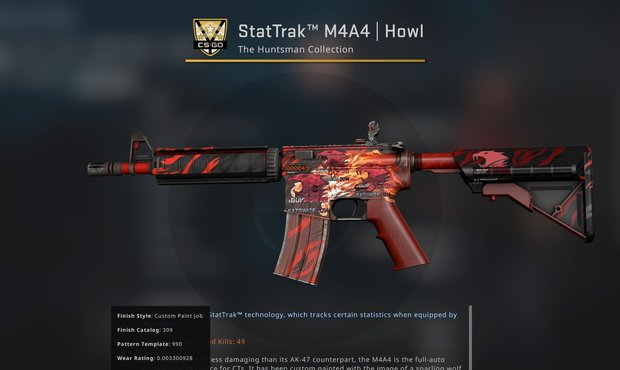
\includegraphics[scale=0.45]{skin.jpg}
\caption{Ukážka jedného skinu na zbraň M4A4}
\label{f:skiny}
\end{figure*}



\section{Žánre počítačových hier} \label{zanre}

Základným problémom je že hry majú mnoho podôb a niekedy je ťažké ich rozlíšiť. Preto má vačšina hier priradených viac žánrov zároveň. V tejto štúdii nájdete viac informácií o niektorách herných žánroch\cite{9618902}. Štúdia o rozdieloch medzi rôznymi hernými žánrami\cite{4561861}.

V diagrame (obrázok~\ref{f:dia}) môžte vidieť základné rozdelenie žánrov, ktoré si neskôr preberieme podrobnejšie.

\pagebreak

\begin{figure*}[h]
\centering
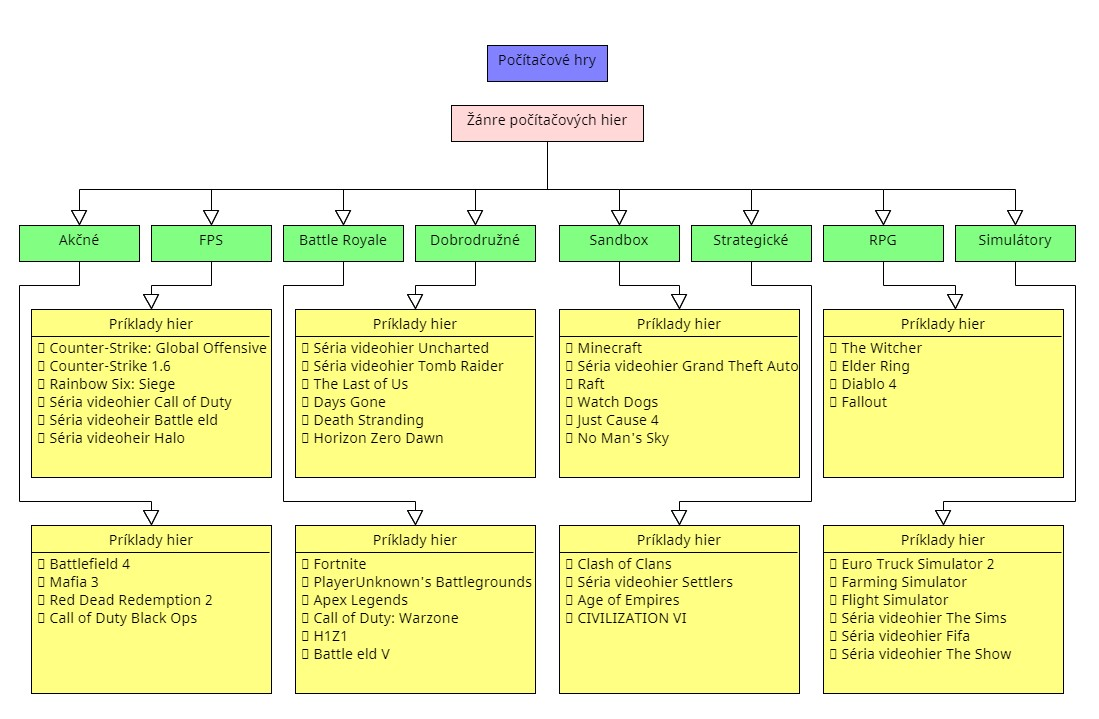
\includegraphics[scale=0.4]{Screenshot_4.jpg}
\caption{Diagram rozdelenia PC hier podľa žánrov}
\label{f:dia}
\end{figure*}

V tabuľke (obrázok~\ref{f:tab}) sú uvedené niektoré novodobé počítačové hry aj s priradenými žánrami, dátumami ich vydania a cenami.

\begin{figure*}[h]
\centering
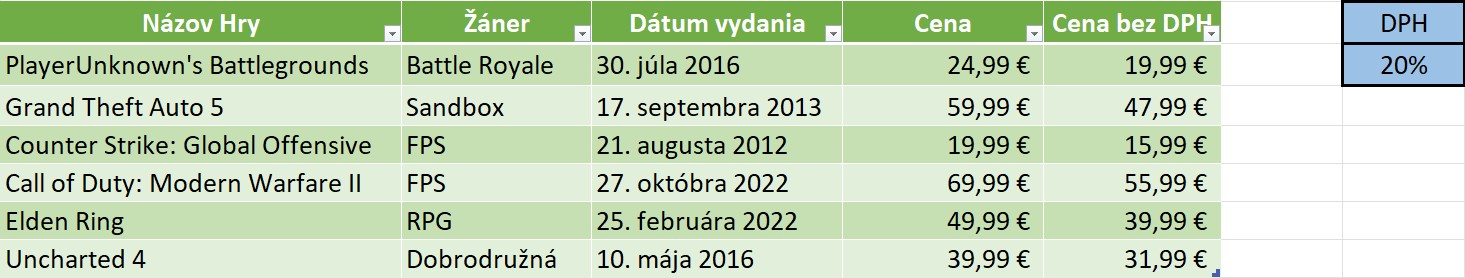
\includegraphics[scale=0.315]{tab.jpg}
\caption{Tabuľka niektorých počítačových hier}
\label{f:tab}
\end{figure*}


Najprv sa pozrieme na akčné hry(časť~\ref{zanre:akcne}), ďalej na FPS (časť~\ref{zanre:fps}) a Battle royale (časť~\ref{zanre:battleroyale}), potom na dobrodružné hry(časť~\ref{zanre:adventure}), a ešet pár ďalších, ako sú Sandbox (časť~\ref{zanre:sandbox}), strategické hry (časť~\ref{zanre:strategicke}), RPG (časť~\ref{zanre:rpg}), a nakoniec simulátory (časť~\ref{zanre:simulatory}).

\subsection{Akčné hry} \label{zanre:akcne}

Patria sem rôzne bojové hry ale aj strielačky. Dôležitou vlastnosťou je mať dobré reflexy pretože hra sa odohráva v reálnom čase, a hráč je pod nátlakom, a má málo času na rozhodovanie. Hráči majú k dispozícii rôzne strelné a tiež ručné zbrane, granáty, nožíky a podobne. Akčné hry sú väčšinou časovo obmedzené. Tento žáner zvyčajne spojený s jedným z ostatných žánrov. Napríklad akčné adventúry alebo akčné RPG. Žánre ktoré vychádzajú z akčných hier sú napríklad FPS alebo Battle Royale. Obrázok s príkladom akčnej hry (obrázok~\ref{f:akcne}, zdroj\footnote{zdroj: https://www.callofduty.com/modernwarfare2}).

\begin{figure*}[tbh]
\centering
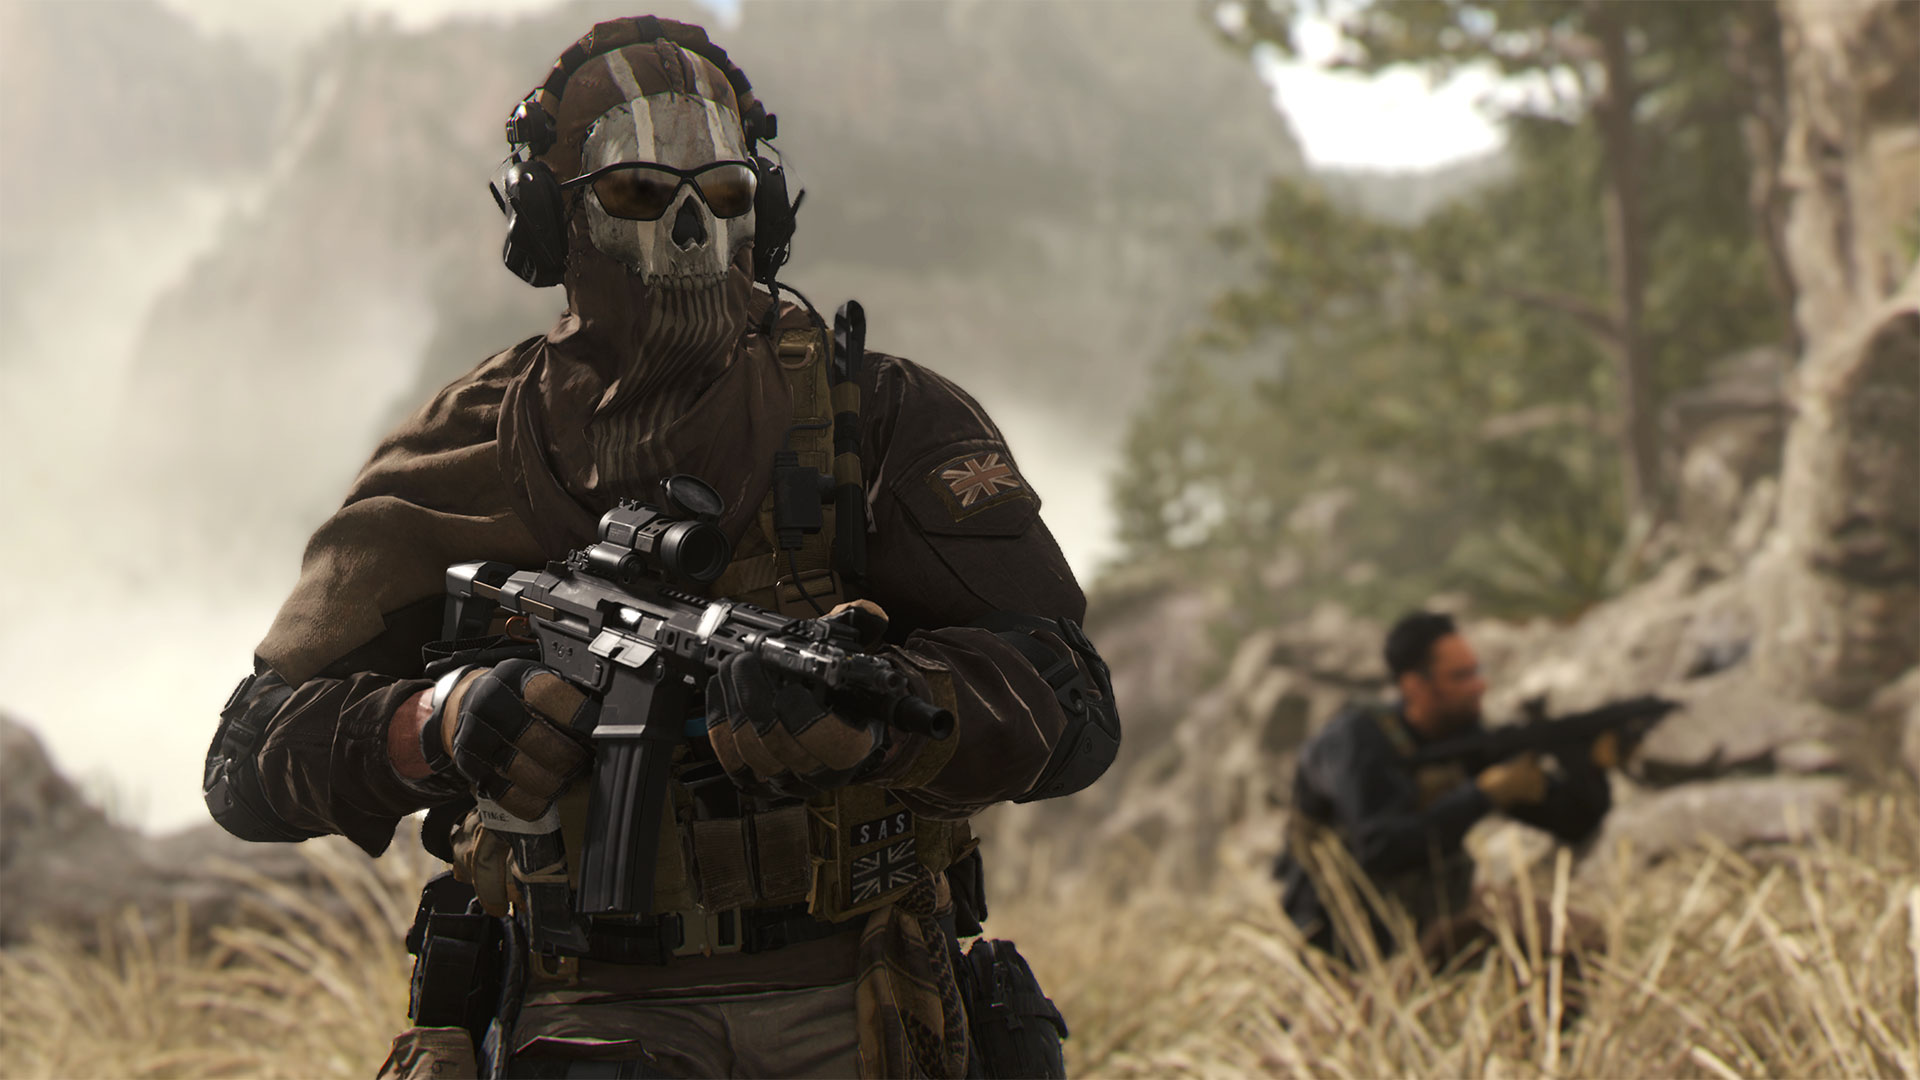
\includegraphics[scale=0.1]{mw2.jpg}
\caption{Obrázok z akčnej hry}
\label{f:akcne}
\end{figure*}



\subsection{FPS} \label{zanre:fps}

First person shooter alebo strielačka z prvého pohľadu je asi najzámejší a najobľúbenejší žáner videohier. Mnohé klasiky ale aj moderné hry spadajú pod tento žáner. V podstate ide o hry, v ktorých hráči hrajú za nejakú postavu a vidia svet z jej pohľadu. Vidia si aj svoje ruky a ostatné časti tela. Hráči majú k dispozícii veľké množstvo strelných a ručných zbraní, a granátov. Je mnoho herných módov ktoré patria do akčných hier, napríklad že sú hráči rozdelení do dvoch tímov, ktoré bojujú proti sebe, alebo každý proti každému s možnosťou respawnu\footnote{po smrti vašej postavy vás hra po určitom čase zase oživí}, alebo hráči bojujú proti botom s umelou inteligenciou. V skratke sú FPS hry všetky hry, v ktorách hráč vidí okolie z pohľadu nejakej hernej postavy, môže ju ovládať, pohybovať sa, má nejaké zbrane a bojuje s nimi proti niekomu inému. Obrázok s príkladom FPS hry (obrázok~\ref{f:csgo}, zdroj\footnote{zdroj:https://www.gosugamers.net/counterstrike/features/54235-cs-go-a-game-that-still-garners-a-high-following}). 

Príklady FPS hier:
\begin{itemize}
\item Counter-Strike: Global Offensive
\item Counter-Strike 1.6
\item Rainbow Six: Siege
\item Séria videohier Call of Duty
\item Séria videoheir Battlefield
\item Séria videoheir Halo
\end{itemize}

\begin{figure*}[ht]
\centering
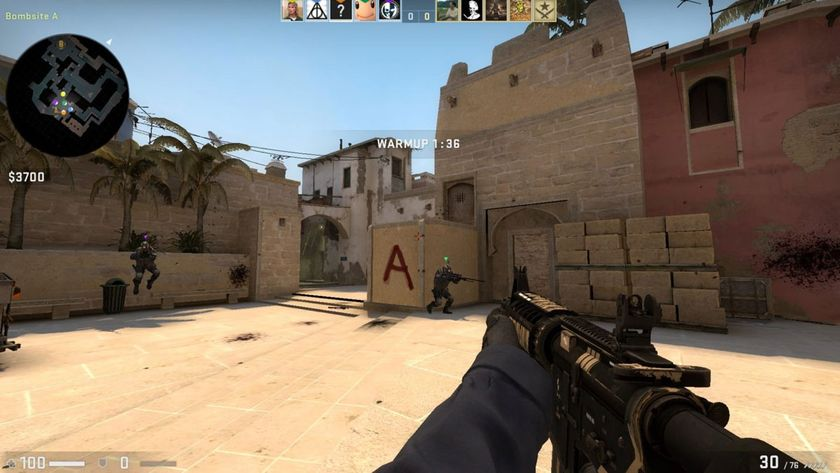
\includegraphics[scale=0.16]{csgo.jpg}
\caption{Screenshot z hry Counter-Strike: Global Offensive}
\label{f:csgo}
\end{figure*}

\subsection{Battle Royale} \label{zanre:battleroyale}

Battle royale hry sú pomerne nový žáner. Sú veľmi podobné akčným hrám, s tým rozdielom, že battle royale hry nemajú príbeh a ide hlavne o to, aby si hráč čo najviac užil a vychutnal akciu. Hlavným znakom je, že hráči bojujú medzi sebou, každý proti každému. Hra sa odohráva na nejakom ostrove alebo na vymedzenej časti pevniny. Nachádza sa tu bezpečná zóna, ktorá je najskôr na celej mape, ale postupne sa zmenšuje a to núti hráčov k častejšiemu stretávaniu a konfliktom. Bezpečná zóna sa zmenšuje dovtedy, kým sú nažive ešte aspoň dvaja hráči. Ak hráč vystúpi z bezpečnej zóny postupne stráca životy a zomiera. Všetci hráči majú dostupnú mapu ostrova s vyznačenými lokalitami a bezpečnou zónou, a prázdny inventár. Každý hráč má na začiatku hry rovanký počet životov a žiadne zbrane. Hra je väčšinou až pre 100 hráčov. Hráči začínajú hru niekde mimo ostrova, a po pripojení všetkých 100 hráčov, sa hráči presunú do lietadla, ktoré letí ponad mapou. Sami sa môžu rozdodnúť kde a kedy vyskočia z lietadla, a pomocou padáku pristanú na ľubovolnom mieste na mape. Po celej mape sú náhodne rozmiesnené zbrane a vozidlá. Cieľom hry je zbierať a vylepšovať rôzne zbrane a zvyšovače životov, liečiť sa, bojovať s ostatnými hráčmi, postupne sa presúvať po mape kvôli zmenšovaniu bezpečnej zóny, prežiť a vyhrať. Hru vyhráva posledný živý hráč. Hra trvá približne 20-30 minút. Obrázok s príkladom Battle royale hry (obrázok~\ref{f:fortnite}, zdroj\footnote{zdroj:https://www.epicgames.com/fortnite/en-US/news/ea-1-6-3-release-notes}).

Príklady Battle royale hier:
\begin{itemize}
\item Fortnite
\item PlayerUnknown's Battlegrounds
\item Apex Legends
\item Call of Duty: Warzone
\item H1Z1
\item Battlefield V
\end{itemize}

\begin{figure*}[h]
\centering
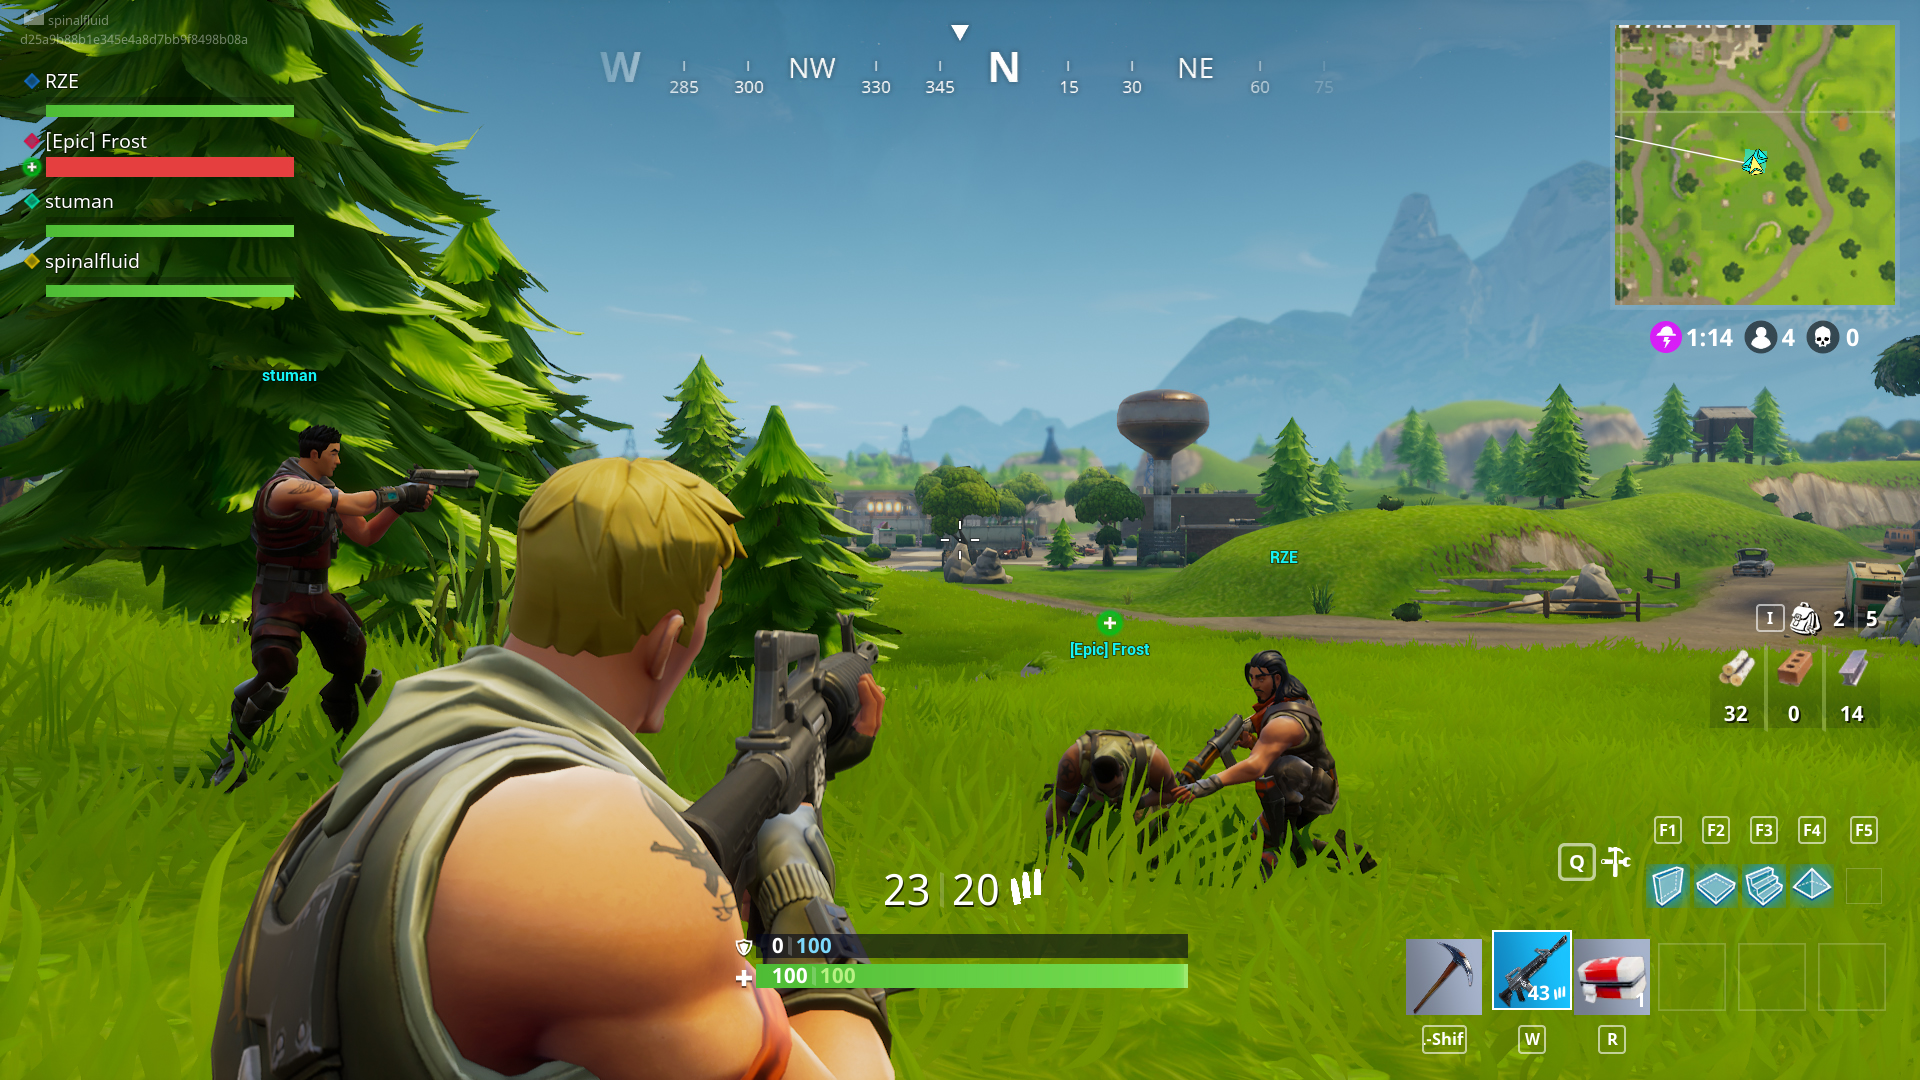
\includegraphics[scale=0.10]{fortnite.jpg}
\caption{Screenshot z hry Fortnite}
\label{f:fortnite}
\end{figure*}

\subsection{Dobrodružné hry} \label{zanre:adventure}

Najskôr mali textovú podobu, no postupne sa vyvíjali až do dnešnej podoby, kde už ide o rozsiahle konverzácie postáv, rôzne zápletky, hádanky a bohatý príbeh. Ide väčšinou o single player hry, ale existujú aj takzvané co-op\footnote{skupina ľudí hrá hru, v ktorej hrajú na rovnakej strane, napríklad proti počítaču}hry. Adventúry majú zvyčajne jednu hlavnú dejovú líniu a veľa vedlajších. Vyskytujú sa v nich aj rôzne easter eggy\footnote{veľkonočné vajíčko je skrytá funkcia alebo nejaký odkaz, minihra, ktorý niekde ukryli autori hry, môže to byť čokoľvek }. Hráč sa posúva v príbehu ďalej interakciou s prostredém, komunikáciou s rôznymi postavami, riešením hádaniek, zbieraním a používaním rôznych predmetov. Väčšinou ide o hry kde sa preskúmavajú hrobky, stratené mestá, hľadá sa poklad a podobne. Hráč sa môže nachádzať aj vo fiktívnom svete plného magických postáv, zvierat a predmetov. ale existujú aj realistické adventúrne hry. Adventúry nemajú na vyhranie kampane žiadny časpvý limit. Obrázok s príkladom dobrodružnej hry (obrázok~\ref{f:uncharted}, zdroj\footnote{zdroj:https://www.polygon.com/guides/21256385/uncharted-4-a-thiefs-end-treasure-collectible-journal-entry-note-conversation}).

Príklady dobrodružných hier:
\begin{itemize}
\item Séria videohier Uncharted
\item Séria videohier Tomb Raider
\item The Last of Us
\item Days Gone
\item Death Stranding
\item Horizon Zero Dawn
\end{itemize}

\begin{figure*}[tbh]
\centering
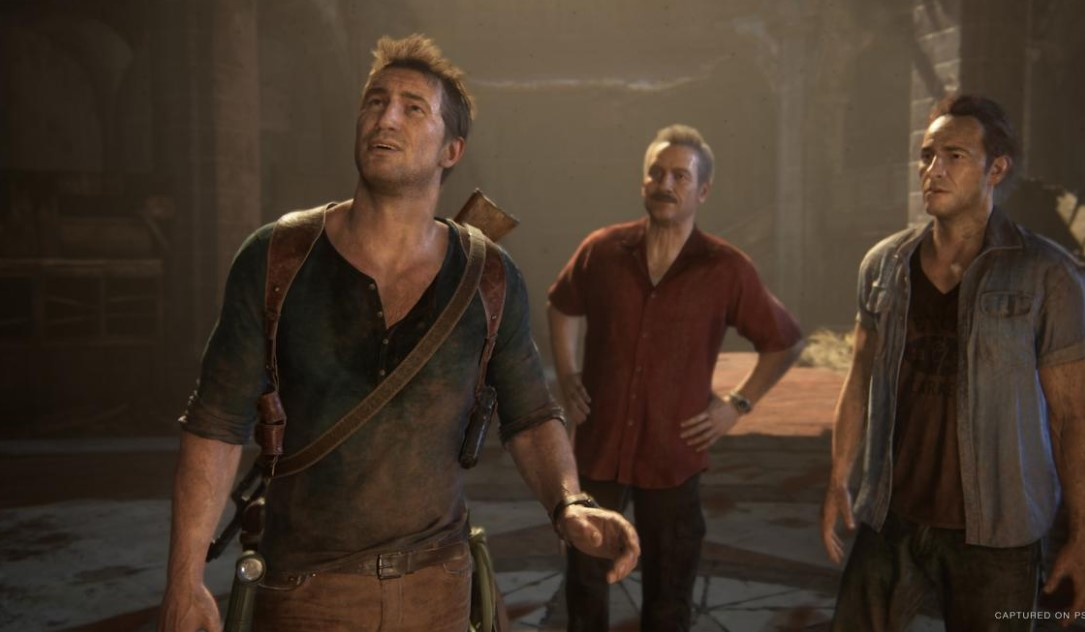
\includegraphics[scale=0.2]{Screenshot.jpg}
\caption{Screenshot z dobrodružnej hry Uncharted 4}
\label{f:uncharted}
\end{figure*}

\pagebreak

\subsection{Sandbox} \label{zanre:sandbox}

Hlavným znakom tohto žánru je otvorený svet, ktorý ponúka svojim hráčom obrovské možnosti na úpravu a tvorbu prostredia. Cieľ si sám kladie hráč, ktorý sa môže slobodne rozhodovať, čo spraví ďalej. Tento žáner podporuje u hráča tvorivosť. Obrázok s príkladom sandbox hry (obrázok~\ref{f:minecraft}, zdroj\footnote{zdroj:https://www.mybasis.com/best-minecraft-survival-mods/}).

Príklady Sandbox hier:
\begin{itemize}
\item Minecraft
\item Séria videohier Grand Theft Auto
\item Raft
\item Watch Dogs
\item Just Cause 4
\item No Man's Sky
\end{itemize}

\begin{figure*}[tbh]
\centering
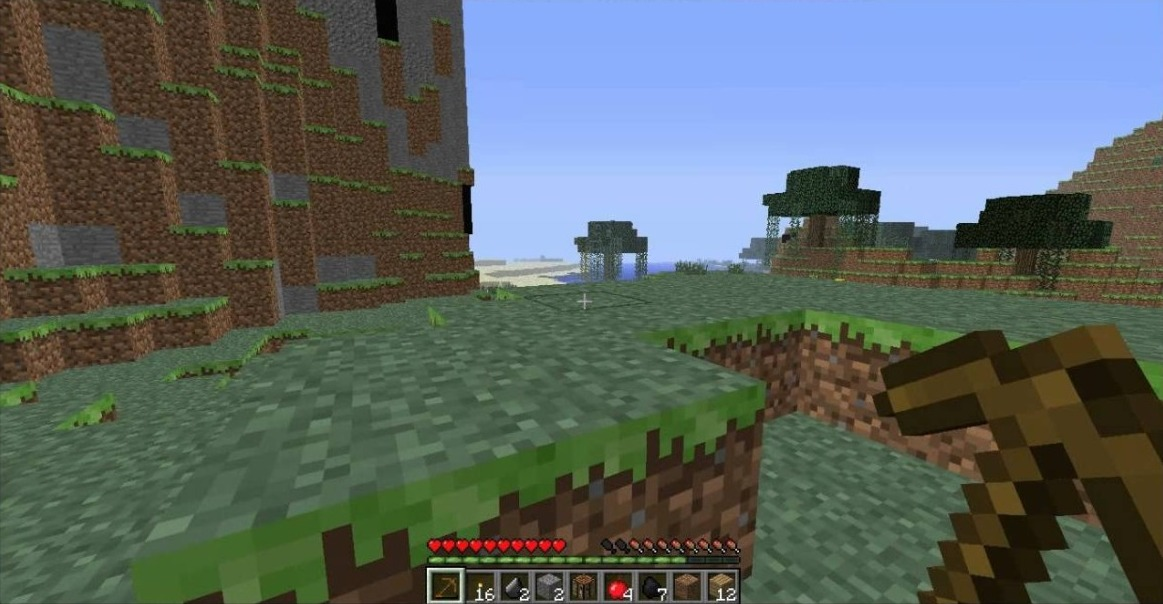
\includegraphics[scale=0.2]{minecraft.jpg}
\caption{Screenshot z hry Minecraft}
\label{f:minecraft}
\end{figure*}

\subsection{Strategické hry} \label{zanre:strategicke}

Sú určené pre hráčov, ktorých baví rôzne plánovanie útokov, vymýšlanie stratégií a rýchle konanie. Cieľom je pomocou svojich bojových zručností, skúseností a dôvtipu vyhrať nad nepriateľom. Hráči svoje ťahy pečlivo plánujú a snažia sa prechytračiť oponenta. Svoju taktiku môžu meniť podľa vývoju hry. Stratégie sú vačšinou zasadené do stredoveku, kde bojujú pomocou vtedajších zbraní. Často má hráč na starosti napríklad nejakú pevnosť alebo kráľovstvo, a jeho úlohou je ju brániť, postupne zlepšovať obranu a hlavne útočiť na pevnosti ostatných hráčov. Tieto hry sú väčinou v online móde, ale môžu mať aj singleplayer mód.  Typickou strategicou hrou je napríklad šach. Obrázok s príkladom strategickej hry (obrázok~\ref{f:coc})



Príklady strategických hier:
\begin{itemize}
\item Clash of Clans
\item Séria videohier Settlers
\item Age of Empires
\item CIVILIZATION VI
\end{itemize}

\begin{figure*}[tbh]
\centering
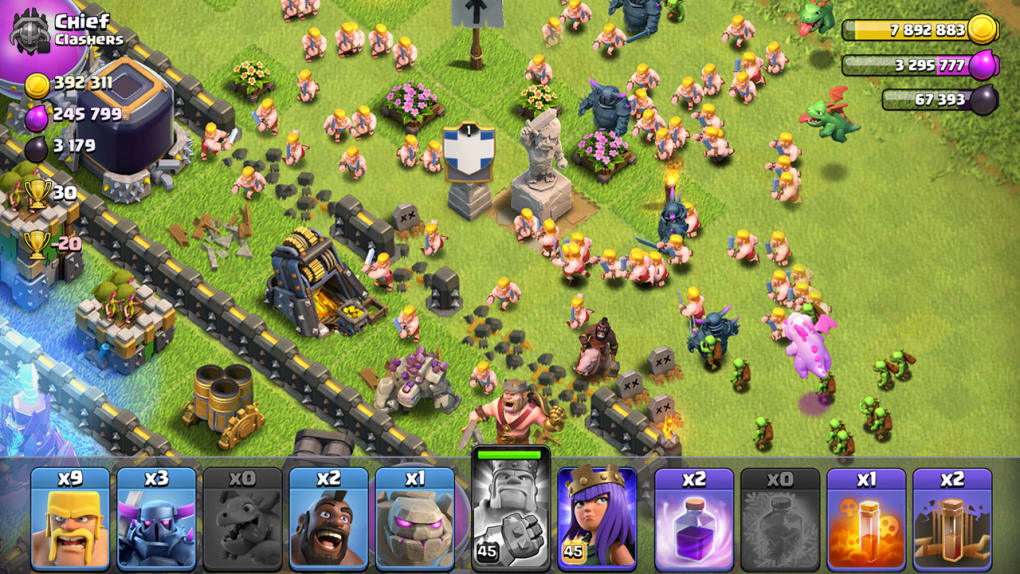
\includegraphics[scale=0.20]{coc.jpg}
\caption{Screenshot z hry Clash of Clans}
\label{f:coc}
\end{figure*}

\subsection{RPG} \label{zanre:rpg}

V RPG hrách (Role Playing Games) sa hráč zväčša pohybuje v rozsiahlej krajine plnej postáv známych z fantasy alebo sci-fi literatúry či rozprávok. Ich hrdinovia, ktorými môžu byť ľudia s bežnými  zamestnaniami, ale aj dobrodruhovia, rytieri či nadprirodzené bytosti, sa v priebehu hry vyvíjajú a v závislosti od vykonávanej činnosti sa zlepšujú ich zručnosti a schopnosti a zväčšuje majetok.(obrázok~\ref{f:rpg})

Príklady RPG hier:
\begin{itemize}
\item The Witcher
\item Elden Ring
\item Diablo 4
\item Fallout
\end{itemize}

\begin{figure*}[h]
\centering
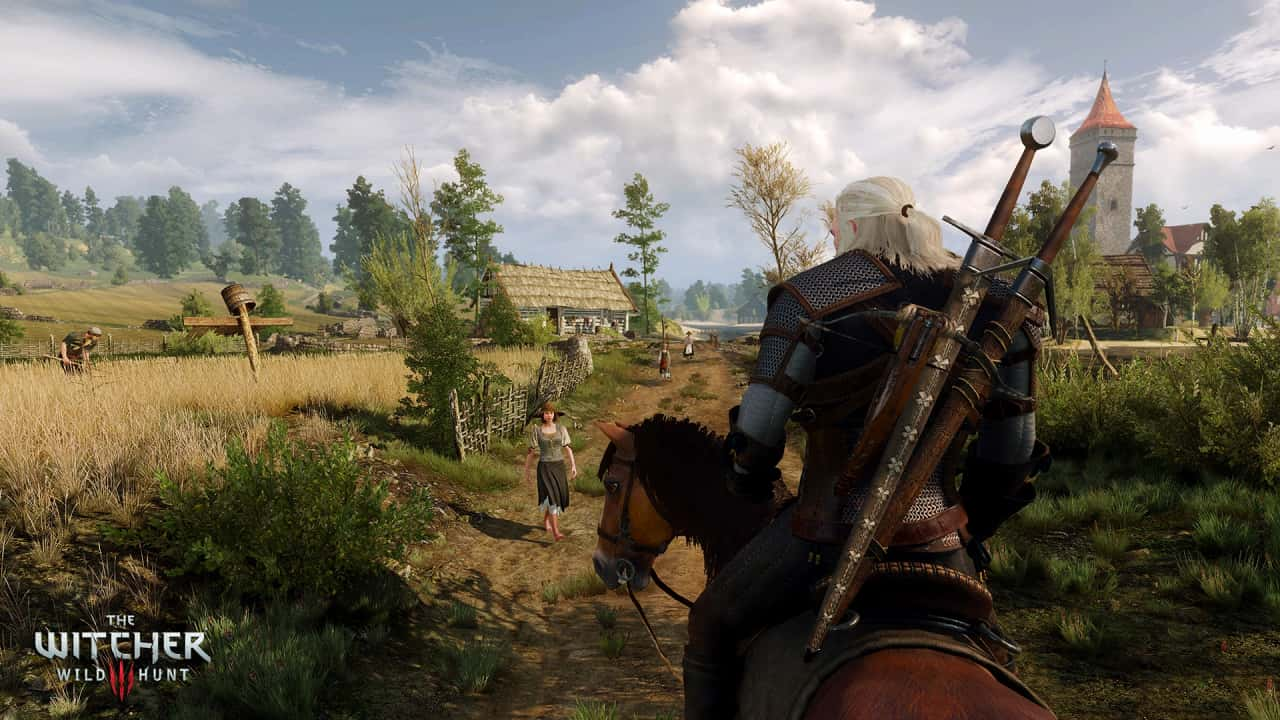
\includegraphics[scale=0.15]{rpg.jpg}
\caption{Screenshot z hry The Witcher}
\label{f:rpg}
\end{figure*}


\subsection{Simulátory} \label{zanre:simulatory}

V týchto hrách ide o simuláciu reálneho života, cieľom je hlavne zabaviť sa, a to spôsobom robenia niečoho, čo v realite buď nemôžeme robiť alebo nevieme robiť a chceme sa to naučiť. Existuje mnoho simulátorov, najznámejšie sú Euro Truck Simulator, Farming Simulator alebo Flight Simulator. V skratke, existuje simulátor skoro na čokoľvek čo sa dá vykonávať v reálnom svete. Nejde o to hru vyhrať, a ani sa nedá vyhrať, ale hrať dovtedy, kým to hráča bude baviť. Obrázok s príkladom sandbox hry (obrázok~\ref{f:ets2}, zdroj\footnote{zdroj:https://www.sector.sk/novinka/244607/euro-truck-simulator-2-dostal-update-138.htm}).

Príklady simulátorov:
\begin{itemize}
\item Euro Truck Simulator 2
\item Farming Simulator
\item Flight Simulator
\item Séria videohier The Sims
\item Séria videohier Fifa
\item Séria videohier The Show
\end{itemize}

\begin{figure*}[h]
\centering
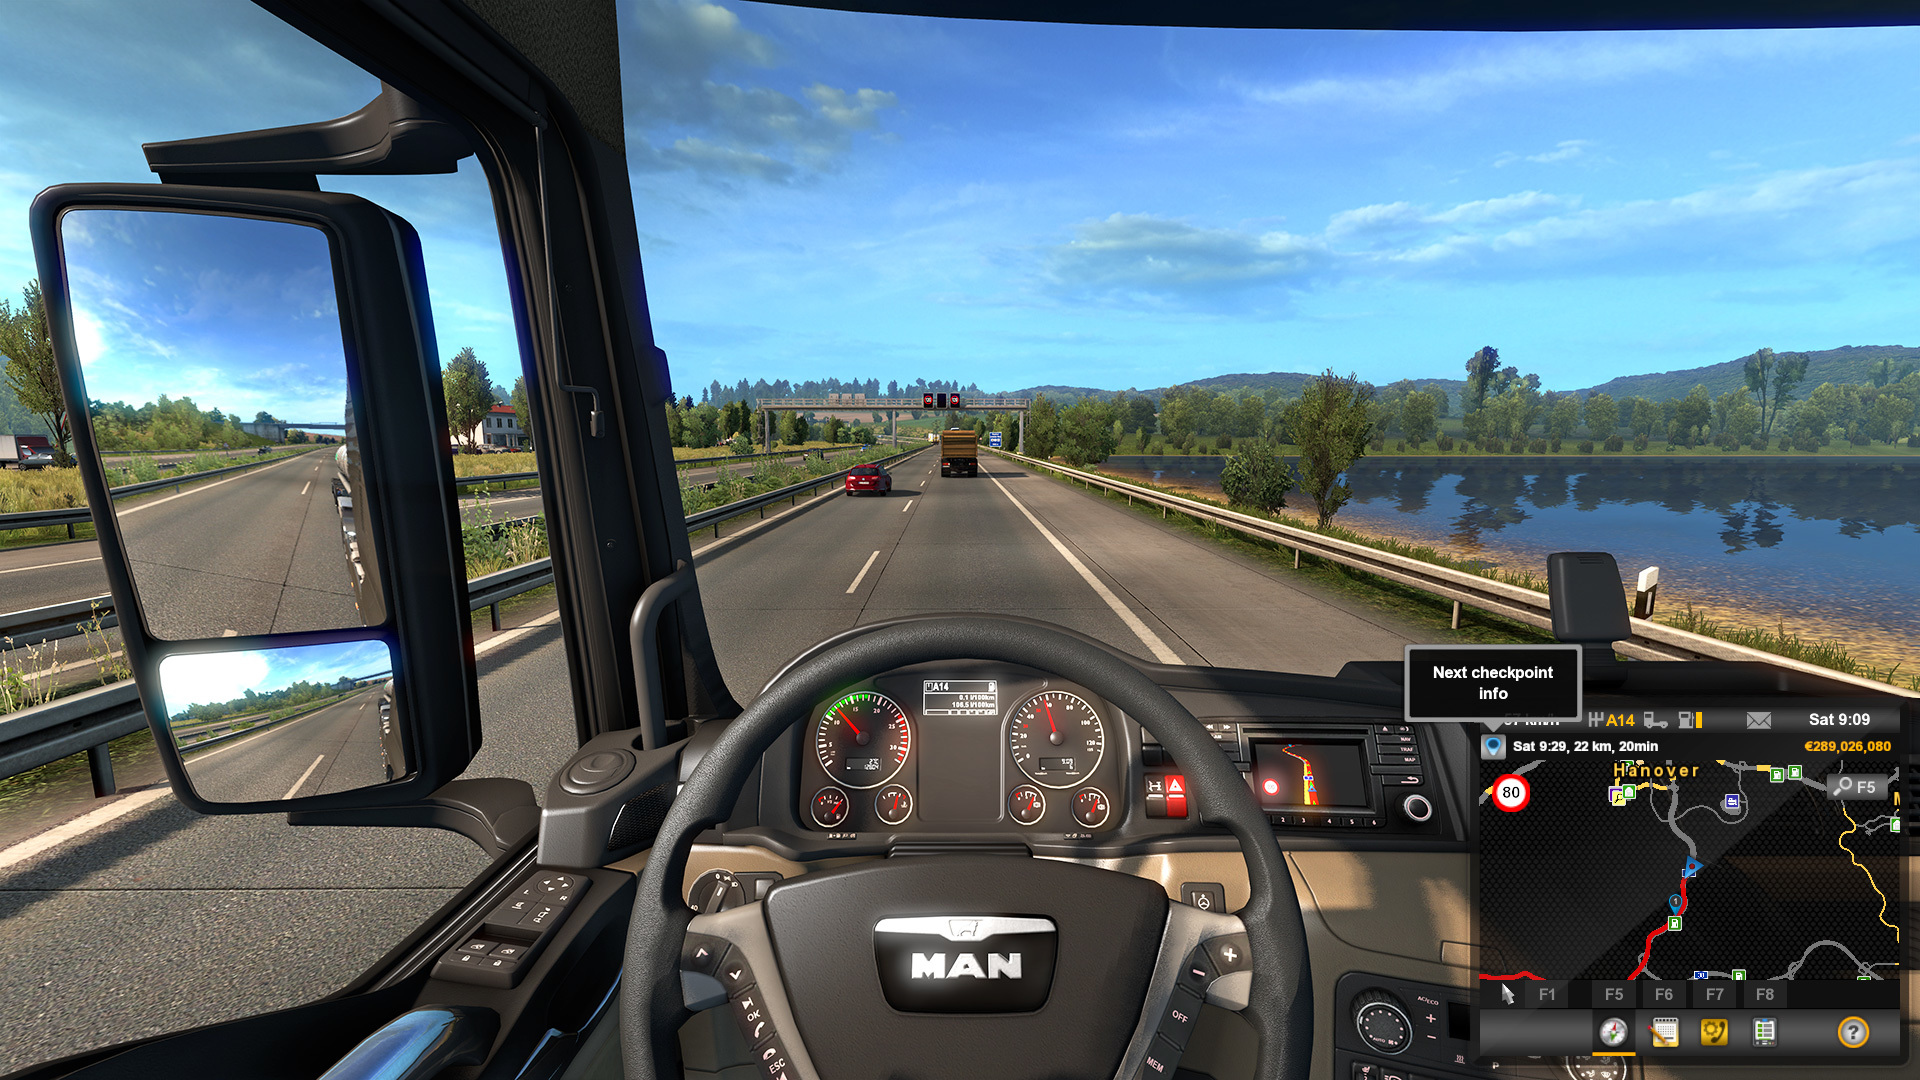
\includegraphics[scale=0.15]{ets.jpg}
\caption{Screenshot z hry Euro Truck Simulator 2}
\label{f:ets2}
\end{figure*}

\pagebreak

\section{Reakcia na témy z prednášok} \label{reakcia}

\paragraph{Spoločenské súvislosti.}

Informatika má potenciál ovplyvniť spoločnosť aj inými spôsobmi. Napríklad používanie algoritmov a umelej inteligencie pri rozhodovaní vyvolalo obavy zo zaujatosti a diskriminácie a rozšírené používanie osobných údajov vyvolalo vážne obavy o súkromie.

\paragraph{Historické súvislosti.}

História informatiky v 21. storočí bola poznačená rýchlym pokrokom technológie a rastúcim významom informácií v našom každodennom živote. Informatika, ktorá zahŕňa využitie technológií na spracovanie a správu informácií, zohrala kľúčovú úlohu pri umožnení tejto transformácie.
Jedným z hlavných pokrokov v histórii informatiky v 21. storočí bolo rozsiahle prijatie internetu a rast World Wide Web. To ľuďom umožnilo prístup a zdieľanie informácií v globálnom meradle a pripravilo pôdu pre nové aplikácie a služby, ktoré zmenili spôsob, akým žijeme a pracujeme.

\paragraph{Technológia a ľudia.}

S rastúcim množstvom generovaných dát a rastúcou závislosťou od technológií je dôležité, aby informatici zvážili dopady svojej práce na ľudí.
Pozitívom je, že informatika má potenciál zlepšiť kvalitu nášho života tým, že zjednoduší a zefektívni úlohy, umožní nám prístup k informáciám a spojenie s ostatnými spôsobmi, ktoré boli predtým nepredstaviteľné. Taktiež otvorila nové príležitosti pre spoluprácu a inovácie a má potenciál pomôcť vyriešiť niektoré z najpálčivejších problémov sveta.
Rýchle tempo technologického pokroku však vyvolalo aj obavy z automatizácie práce a potenciálu, aby sa technológie využívali škodlivými spôsobmi. Je dôležité, aby informatici zvážili tieto potenciálne negatívne vplyvy a snažili sa ich zmierniť.

\paragraph{Udržateľnosť a etika.}

Udržateľnosť v informatike zahŕňa používanie technológie spôsobom, ktorý je zodpovedný za životné prostredie a nevyčerpáva zdroje ani neprispieva ku klimatickým zmenám. To môže zahŕňať používanie energeticky účinných technológií, implementáciu programov recyklácie elektronického odpadu a zváženie vplyvu dátových centier na životné prostredie.
Etika v informatike zahŕňa zabezpečenie toho, aby sa technológie používali spôsobom, ktorý je spravodlivý, zodpovedný a rešpektuje práva jednotlivcov. To môže zahŕňať ochranu súkromia používateľov, vyhýbanie sa zaujatosti v algoritmoch a zvažovanie potenciálnych dôsledkov technológie na spoločnosť.



\section{Záver} \label{zaver}

To, že sa počítačové hry z roka na rok menia a vylepšujú, nie je pre vás určite novinkou. Vidieť ich však v rozmedzí mnoho rokov je zaručene niečo neopísateľné. Počítačová technika ide neuveriteľne rýchlo dopredu. Tieto hry sú s nami iba pár desiatok rokov, ale za tú dobu sa stihli výrazne zmeniť. Od jednoduchých pixelov na čiernobielych monitoroch sme sa dostali k prepracovanej grafike, ktorá nielen verne zachytáva našu skutočnosť, ale dokáže vykresliť aj neskutočnosť. Napríklad fantastické svety ktoré existujú len vo videohrách.


Hry majú mnoho podôb a niekedy je ťažké ich rozlíšiť. Väčšina hier má viac žánrov zároveň. Je ťažké vytvoriť hru len s jedným žánrom. Vždy sa v nej nájdu prvky aj z ostatných. Niekedy viac, inokedy menej.



%\input{example.tex}



%\acknowledgement{Ak niekomu chcete poďakovať\ldots}


% týmto sa generuje zoznam literatúry z obsahu súboru literatura.bib podľa toho, na čo sa v článku odkazujete
\bibliography{literatura}
\bibliographystyle{alpha} % prípadne alpha, abbrv alebo hociktorý iný
\end{document}
